\section{App management}
\label{sec:app_management}

\subsection{Requirements}
\label{sec:appman_requirements}

As shown in \autoref{fig:state_diagram} in \autoref{sec:design_overview}, the ``no app selected''-state and the ``no child selected''-state are the states which the launcher is in when the user is about to launch a \giraf[] app. \\

\noindent Three pieces of information are needed in order to launch an app:

\begin{enumerate}
	\item Current authenticated guardian
	\item App to launch
	\item Selected child to launch the app with
\end{enumerate}

The first requirement is already given, since the launcher cannot be in any of the two states without the user already being authenticated.
The second requirement is straightforward, as it is not possible to launch an app without knowing which app to launch.
The first and third requirements are needed in order to fulfill the services which the launcher needs to have in order to be a functional part of the \giraf[] platform, as shown in \autoref{fig:external_architecture}.

Furthermore, additional pieces of information must be known to the user:

\begin{enumerate}
	\item Date, including week number
	\item Network status 
\end{enumerate}

As the \giraf[] platform is thought to be the primary electronic tool of guardians, the current date and weeknumber is provided.
Since the \giraf[] platform uses both local and remove storage, there might be latency in synchronizing these storages, and therefore it is important for the user to know if the both storages are synchronized or not.

Since the \giraf[] platform should be flexible and customizable, it must be possible to change color of the \giraf[] icons.

\subsection{Solution}
\label{sec:appman_solution}

\autoref{fig:appmanagement_design} shows the flowchart over the interactions the user can perform, and the actions the launcher takes upon the interactions, in order to fullfill the requirements listed in \autoref{sec:appman_requirements}.

\begin{figure}[h]
	\centering
	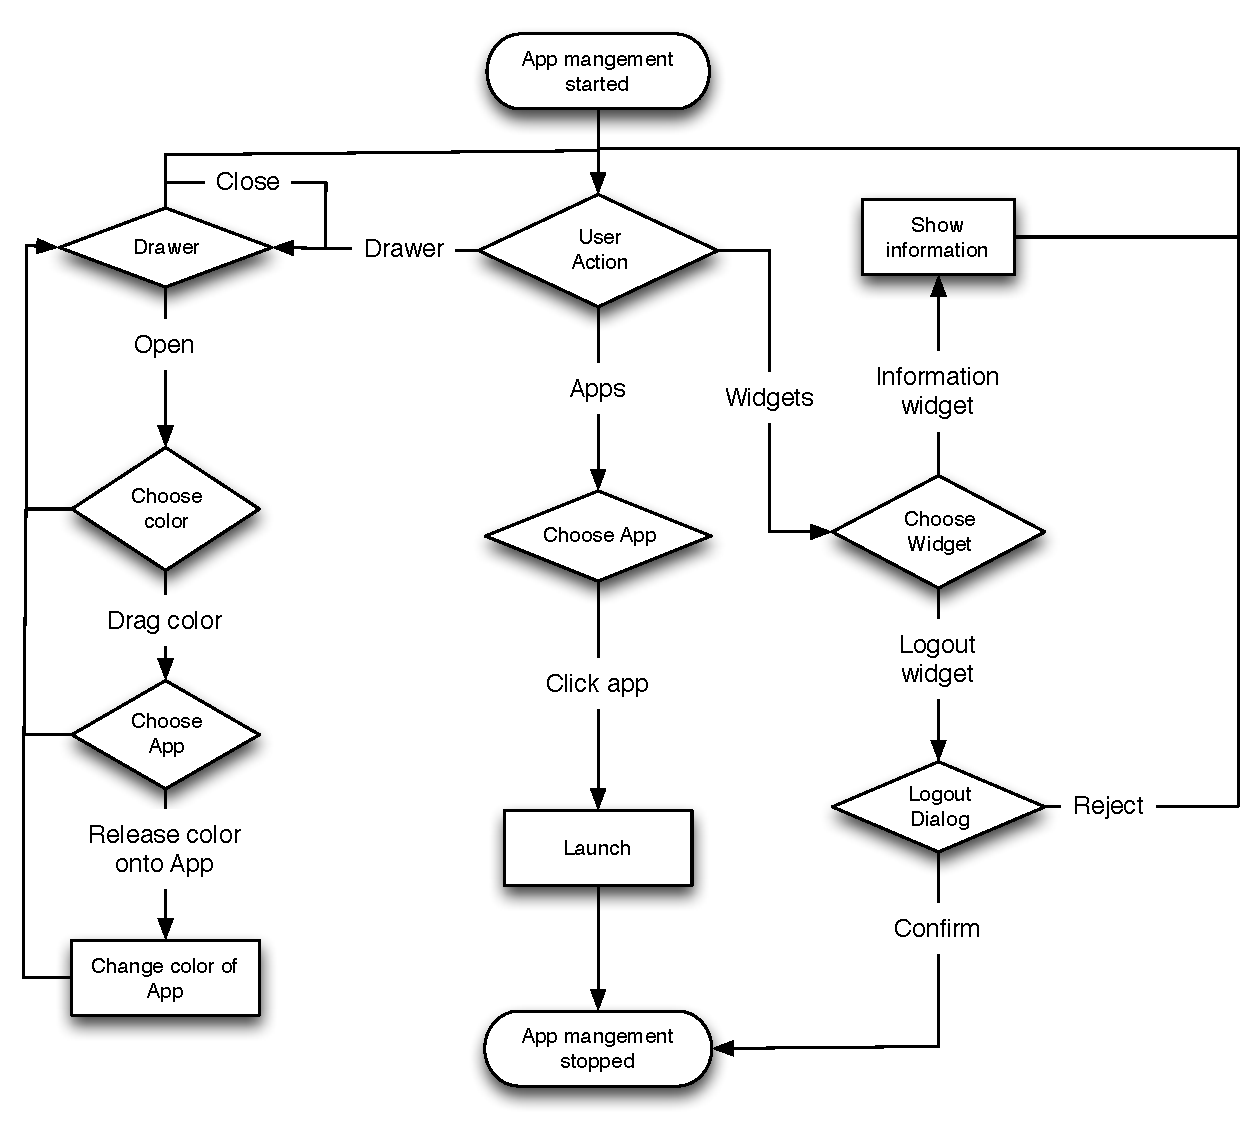
\includegraphics[width=1\textwidth]{gfx/appmanagement.pdf}
	\caption{Flowchart over the app management functionality}
	\label{fig:appmanagement_design}
\end{figure}

\autoref{fig:appmanagement_design} shows three branches of interactions and actions:

\begin{itemize}
	\item Change app settings
	\item Launch app
	\item Request information
\end{itemize}






\subsubsection{The drawer}
\label{sec:drawer}
The drawer is a place to put functionality. As seen in \autoref{fig:appmanagement_design} everything that have to do with change app settings have to do with something in the drawer.
\paragraph{Widgets}
\label{par:widgets}
Widgets in the \giraf[] system helps the user request information. As seen in \autoref{fig:appmanagement_design} the user can take the action to request information. If the user choose an information the information will be selected and shown to the user.

\paragraph{Color picker}
\label{par:colorpicker}
